%//==============================--@--==============================//%
\section{Ondas Planas}
\label{sec:ondas-planas}

%//==============================--@--==============================//%
\subsection{Equações de Onda livres de Fontes}
\label{sec:eq-onda-sem-fonte}

Para meios isotrópicos padrão (sem dispersão), numa região isenta de fontes onde  $\rho = 0$ e $\mathbf{J}_{ext} = 0$, as equações de Maxwell podem ser reescritas da seguinte forma:
\begin{align}
    \nabla\times \mathbf{E} &= -\mu\,\frac{\partial \mathbf{H}}{\partial t} & \nabla\times \mathbf{H} &= \epsilon\,\frac{\partial \mathbf{E}}{\partial t}\label{eq:1} \\
    \nabla\cdot \mathbf{E} &= 0 & \nabla\cdot \mathbf{H} &= 0\label{eq:2}
\end{align}

As equações diferenciais de primeira ordem podem ser unificadas numa única equação diferencial de segunda ordem, em $\mathbf{E}$ ou em $\mathbf{H}$. Aplicando o rotacional a (\ref{eq:1}) obtemos:
\begin{equation}
        \nabla \times (\nabla \times \mathbf{E}) = -\mu\,\dfrac{\partial}{\partial t}\left(\nabla \times \mathbf{H}\right)
\end{equation}
Por conseguinte, substituindo com a equação par em (\ref{eq:1}), obtemos:
\begin{equation}
    \nabla\times (\nabla \times \mathbf{E}) = -\mu\epsilon\,\frac{\partial^2 \mathbf{E}}{\partial t^2}
\end{equation}
Com recurso à identidade vetorial e admitindo a equação (\ref{eq:2}), é possivel reescrever:
\begin{equation}
     \nabla \times (\nabla \times \mathbf{E}) = \nabla(\nabla\cdot\mathbf{E}) - \nabla^2\mathbf{E} = - \nabla^2\mathbf{E}
\end{equation}
Finalmente obtemos:
\begin{equation} \label{eq:wave-eq}
    \boxed{\nabla^2\mathbf{E} -\mu\epsilon\,\frac{\partial^2 \mathbf{E}}{\partial t^2} = 0}
    \quad\text{e de forma análoga}\quad
    \boxed{\nabla^2\mathbf{H} -\mu\epsilon\,\frac{\partial^2 \mathbf{H}}{\partial t^2} = 0}
\end{equation}

\vspace{-0.75em}
\begin{warning}
    A equação de onda é de segunda ordem, nas coordenadas temporais e espaciais. Utilizamos $\nabla^2$ para representar o operador \emph{Laplaciano}; podemos, portanto, escrever as equações de \eqref{eq:wave-eq} em cada coordenada do campo.
\end{warning}

Uma equação de onda \underline{unidimensional} genérica tem a forma e solução como se apresenta:
$$
    \frac{\partial^2 \mathbf{u}}{\partial x^2} - \frac{1}{c^2} \frac{\partial^2 \mathbf{u}}{\partial t^2} = 0
    \;\implies\;
    \boxed{%
        \mathbf{u} = f(x - ct) + g(x + ct)
    }
    \quad \text{(variação espacial em apenas uma das direções)}
$$

%//==============================--@--==============================//%
\subsection{Regime Harmónico no Tempo}

Dado que as equações de Maxwell são equações diferenciais lineares, variações temporais sinusoidais impostas pelo gerador de funções com uma frequência específica produzirão variações sinusoidais de $\mathbf{E}$ e $\mathbf{H}$ com a mesma frequência no estado estacionário.

O campo elétrico $\mathbf{E}(\mathbf{r}, t) $ em regime harmónico pode ser reescrito em termos da amplitude complexa na forma de fasor $\underline{\mathbf{E}}(\mathbf{r})$ na forma:
\begin{equation}
    \mathbf{E}(\mathbf{r}, t) = \Re\left\{\underline{\mathbf{E}}(\mathbf{r}) e^{j\omega t}\right\}
\end{equation}
As amplitudes complexas dos campos satisfazem as equações de Maxwell independentes do tempo:
\begin{equation}
    \nabla\times\underline{\mathbf{E}} = -j\omega\underline{\mathbf{B}}\qquad
     \nabla\times\underline{\mathbf{H}} = \underline{\mathbf{J}}_{ext} + j\omega\underline{\mathbf{D}}
\end{equation}
e por conseguinte
\begin{equation}\label{eq:time-independent-max}
    \boxed{\nabla\times\underline{\mathbf{E}} = -j\omega\mu\underline{\mathbf{H}}\qquad
     \nabla\times\underline{\mathbf{H}} = \underline{\mathbf{J}}_{ext} + j\epsilon\omega\underline{\mathbf{E}}}
\end{equation}

%//==============================--@--==============================//%
\subsection{Propriedade das Ondas Planas}
As ondas planas são a solução mais simples das equações de Maxwell. Por definição, um campo de onda plana é descrito por:
\begin{equation}
    \underline{\mathbf{E}} = \underline{\mathbf{E}}_0\, e^{-j \mathbf{k}\cdot\mathbf{r}}\qquad
    \underline{\mathbf{H}} = \underline{\mathbf{H}}_0\, e^{-j \mathbf{k}\cdot\mathbf{r}}
\end{equation}
O termo $e^{-j \mathbf{k}\cdot\mathbf{r}}$ é conhecido como fator de propagação, pois determina a variação espacial dos campos. É expresso em termos das coordenadas do ponto de observação $\mathbf{r} = (x, y, z)$ e em termos do vetor de onda fundamental $\mathbf{k} = (k_x, k_y, k_z)$.

É conveniente escrever o fator de propagação em termos de um vetor unitário $\mathbf{\hat{d}}$ e um fator k denominado número de onda. Em meios isotrópicos, $\mathbf{\hat{d}}$ determina a direção de propagação da onda.
\begin{equation}
    \boxed{e^{-j \mathbf{k}\cdot\mathbf{r}} = e^{-j k\,\mathbf{\hat{d}}\cdot\mathbf{r}}}
\end{equation}
O comprimento de onda $\lambda$ é a distância pela qual a fase da onda sinusoidal muda por $2\pi$ radianos. Uma vez que o fator de propagação $e^{-j k\,\mathbf{\hat{d}}\cdot\mathbf{r}}$ acumula uma fase de $k$ radianos por metro, temos por definição que $k\lambda = 2\pi$. O comprimento de onda $\lambda$ pode ser expresso através da frequência da onda em hertz, $f = \omega/2\pi$, como se segue:
\begin{equation}
    \boxed{\lambda = \frac{2\pi}{k} = \frac{c}{f}}
\end{equation}

\begin{warning}
    Se o meio de propagação for o espaço livre, usamos os valores de vácuo dos parâmetros $\{\epsilon, \mu, c, \eta\}$, ou seja, $\{\epsilon_0, \mu_0, c_0, \eta_0\}$. O comprimento de onda no espaço livre e o número de onda correspondente são:
    \begin{equation}
        \lambda_0 = \frac{2\pi}{k_0} = \frac{c_0}{f} , \quad k_0 = \frac{\omega}{c_0}  
    \end{equation}
    Num dielétrico com índice de refração $n = \sqrt{\epsilon_r\mu_r}$, a velocidade da luz $c$, o comprimento de onda $\lambda$ e a impedância característica $\eta$ são todos reduzidos por um factor de $n$ em comparação com os valores no espaço livre, enquanto que o número de onda $k$ é aumentado por um factor de $n$:
    \begin{equation}
        c = \dfrac{c_0}{n}, \quad\eta = \dfrac{\eta_0}{n}, \quad\lambda = \dfrac{\lambda_0}{n}, \quad k = nk_0
    \end{equation}
\end{warning}

%//==============================--@--==============================//%
\clearpage
\subsection{Ondas Planas em Meios sem Perdas} \label{sec:ondas-sem-perdas}

Em materiais uniformes não dispersivos, com $\epsilon, \mu$ independentes de $\mathbf{r} = (x, y, z)$. As ondas planas satisfazem as equações de Maxwell sem fonte ($\mathbf{J} = 0$), definidas em (\ref{eq:time-independent-max}).

A variação no espaço de uma onda plana é controlada pelo fator de propagação $e^{-j \mathbf{k}\cdot\mathbf{r}}$. Assim:
\begin{equation}
    \begin{aligned}
        \nabla \times \mathbf{\underline{E}} &= \left( \frac{\partial}{\partial x}, \frac{\partial}{\partial y}, \frac{\partial}{\partial z} \right)  \times
         \left(\mathbf{\underline{E}}_0 e^{-j\mathbf{k}\cdot \mathbf{r}}\right) = \\[2pt]
         &=
         \left( \frac{\partial}{\partial x}, \frac{\partial}{\partial y}, \frac{\partial}{\partial z} \right)
         \times
         \left(\underline{E}_x,\underline{E}_y,\underline{E}_z\right) =
         \left(
             \frac{\partial \underline{E}_z}{\partial y} - \frac{\partial \underline{E}_y}{\partial z}, 
             \frac{\partial \underline{E}_x}{\partial z} - \frac{\partial \underline{E}_z}{\partial x},
             \frac{\partial \underline{E}_y}{\partial x} - \frac{\partial \underline{E}_x}{\partial y}
         \right)
    \end{aligned}
\end{equation}
Recorrendo ao cálculo das derivadas em todas as componente:
\begin{equation}
    -j\eqnmarkbox[blue]{curl}{\left(
     \underline{E}_{0z} k_y - \underline{E}_{0y} k_z,
     \underline{E}_{0x} k_z - \underline{E}_{0z} k_x,
     \underline{E}_{0y} k_x - \underline{E}_{0x} k_y
    \right)} \cdot e^{-j\mathbf{k}\cdot \mathbf{r}}
\end{equation}

\annotate{below, right}{curl}{$(k_x,k_y,k_z)\times(\underline{E}_{0x},\underline{E}_{0y},\underline{E}_{0z})$}
\noindent Consequentemente,
\begin{equation}
     \boxed{-j\mathbf{k}\times\underline{\mathbf{E}}_0\,e^{-j\mathbf{k}\cdot \mathbf{r}} = -j\mathbf{k}\times\mathbf{\underline{E}}}
\end{equation}
É então possível reescrever as equações de Maxwell:
\begin{equation}\label{eq:Max-k}
    \boxed{\mathbf{k}\times\mathbf{\underline{E}} =\omega\mu\mathbf{\underline{H}}\qquad
    \mathbf{k}\times\mathbf{\underline{H}} = -\omega\epsilon\mathbf{\underline{E}}}
\end{equation}
\begin{check}
    A equação à esquerda implica que $\mathbf{H}$ é perpendicular a ambos $\mathbf{k}$ e $\mathbf{E}$. Similarmente, a equação à direita mostra que $\mathbf{E}$ é perpendicular a ambos $\mathbf{k}$ e $\mathbf{H}$. Assim, os três vetores são mutuamente perpendiculares e dizemos que a onda é eletromagnética transversal (\textit{transverse electromagnetic}, TEM). Formalmente podemos escrever:

    \begin{equation}
        \mathbf{k}\cdot\mathbf{\underline{E}} = \mathbf{k}\cdot\mathbf{\underline{H}} = 0\qquad\mathbf{\underline{E}}\cdot\mathbf{\underline{H}} = 0
    \end{equation}
\end{check}
Os vetores $\mathbf{\underline{E}},\, \mathbf{\underline{H}},\, \mathbf{k}$ ou, analogamente\footnote{É conveniente escrever o vetor de onda em termos de um vetor unitário (ou versor) $\mathbf{\hat{d}}$ e um escalar $k$: $\mathbf{k} = k\mathbf{\hat{d}}.$ O escalar $k$ é o número de onda. Em meios isotrópicos padrão, o vetor $\mathbf{\hat{d}}$ determina a direção de propagação da onda.~\cite{silveirinha2023}}, $\mathbf{\underline{E}},\, \mathbf{\underline{H}},\, \mathbf{\hat{d}}$ formam uma base direita do espaço. As oscilações do campo são prependiculares à direção de propagação.

\vspace{-0.75em}
\begin{minipage}[c]{0.35\linewidth}
    \begin{figure}[H]
        \centering
        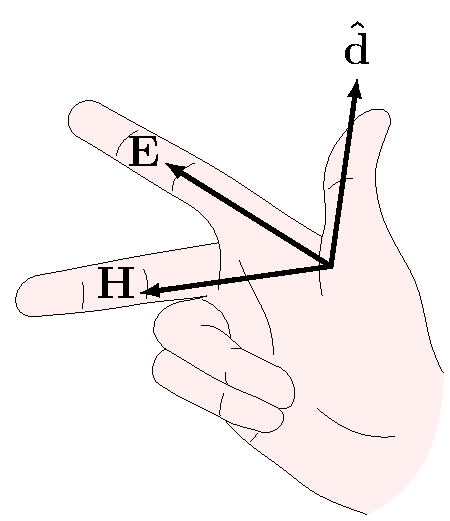
\includegraphics[width=0.75\linewidth]{img/1/Right-hand-basis.pdf}
        \caption{Base direita do espaço.}
    \end{figure}
\end{minipage}\hfill
\begin{minipage}[c]{0.65\linewidth}
    Substituindo $k = \omega\sqrt{\mu\epsilon} = n \cdot \omega/c $ em \eqref{eq:Max-k} e utilizando $k = \mathbf{k}\cdot\mathbf{\hat{d}}$, obtemos a seguinte relação explícita entre os campos e a direção de propagação da onda:
    \begin{equation}
        \boxed{ \mathbf{H} = -\frac{1}{\eta}\mathbf{\hat{d}} \times \mathbf{E}, \quad \mathbf{E} = \eta\mathbf{H} \times \mathbf{\hat{d}} }
    \end{equation}
    O produto vetorial roda efetivamente o campo relevante por 90°.
    \begin{warning}
        Esta relação é sempre válida para ondas planas em meios uniformes não dispersivos!
    \end{warning}
\end{minipage}

\vspace{0.5em}
A ligação entre a frequência angular e o número de onda implica que também existe uma ligação entre os períodos de tempo e espaço da onda. Podemos escrever:

\vspace{0.5em}
\begin{equation}
    \frac{\eqnmarkbox[blue]{T}{T}}{\lambda} = \frac{2\pi}{\omega} = \frac{2\pi}{k}\,\frac{n}{c} = \eqnmarkbox[red]{S}{\lambda}\, \frac{n}{c}
\end{equation}

\annotate{above, label below}{T}{período temporal}
\annotate{below, label above}{S}{período espacial}

%//==============================--@--==============================//%
\clearpage
\begin{question}
    Considere uma onda plana que se propaga pelo vácuo, descrita por:
    \begin{equation*}
        \mathbf{\underline{E}} = \mathbf{\underline{E}}_0 e^{j k_0 y}, \quad \text{onde}\; \mathbf{\underline{E}}_0 = E_0 \mathbf{\hat{x}}
    \end{equation*}
    Determine o campo magnético da onda no domínio do tempo.
    
    \questionSep
    \textbf{Solução}: O campo elétrico instantâneo pode ser calculado através de:
    $$
        \mathbf{E}(y,\,t) = \Re\{\mathbf{\underline{E}} e^{j\omega t}\} = E_0\mathbf{\hat{x}}\cos(\omega\,t + k_0 y)
    $$
    Por conseguinte, sabemos que a relação explicita entre os campos e a direção de propagação é dada por:
    $$
        \mathbf{H} = -\frac{1}{\eta_0}\mathbf{\hat{d}} \times \mathbf{E}
    $$
    Tomando a fórmula do fator de propagação, $e^{-jk_0\mathbf{r}\cdot \mathbf{\hat{d}}}$, é possível escrever:
    $$
        \begin{aligned}
               -\mathbf{r}\cdot\mathbf{\hat{d}} &= y\\
               -(x,\,y,\,z)\cdot (d_x,\,d_y,\,d_z) &= \eqnmarkbox[blue]{dot_p}{-xd_x - yd_y - zd_z}\\
        \end{aligned}
    $$
    \annotate[yshift=1em]{above}{dot_p}{para qualquer ($x,\,y,\,z$)}
    
    \vspace{-1.25em}
    Por inspeção direta, sabendo que $\mathbf{\hat{d}}$ é um versor, obtemos:
    $$
        \begin{cases}%
            d_x = 0\\
            d_y = -1\\
            d_z = 0
        \end{cases}\rightarrow\,
        \boxed{\mathbf{\hat{d}} = -\mathbf{\hat{y}}}
    $$
    Logo,
    $$
        \begin{aligned}
                \mathbf{H}(y,\,t) &= -\frac{1}{\eta_0}\mathbf{\hat{y}} \times \mathbf{E}(y,\,t)\\
                &= -\frac{1}{\eta_0}\mathbf{\hat{y}} \times \left[ E_0\mathbf{\hat{x}}\cos(\omega\,t + k_0 y) \right]\\
                &= \boxed{\frac{1}{\eta_0}E_0\mathbf{\hat{z}}\cos(\omega\,t + k_0 y)} 
        \end{aligned}
    $$
    \qed
\end{question}

%//==============================--@--==============================//%
\subsection{Ondas Planas em Meios com Perdas} \label{sec:ondas-com-perdas}

Vimos \hyperref[sec:material-generico-dispersivo]{anteriormente} que as perdas de potência podem surgir devido à condução e/ou polarização no material. Uma onda que se propaga num meio com perdas estabelecerá uma corrente de condução e uma corrente de deslocamento (polarização), onde ambas causam perdas óhmicas.

Podemos extender a discussão da \hyperref[sec:ondas-sem-perdas]{secção anterior} considerando os resultados obtidos em \ref{sec:material-generico-dispersivo}, nomeadamente:
\begin{equation}
    \epsilon(\omega) = \epsilon_d(\omega) + \frac{\sigma_c(\omega)}{j\omega}
\end{equation}
\begin{equation}
    \nabla \times \mathbf{\underline{E}} = -j\omega\mu(\omega)\mathbf{\underline{H}},
    \quad
    \nabla \times \mathbf{\underline{H}} = j\omega\epsilon(\omega)\mathbf{\underline{E}}
\end{equation}
para uma região no espaço isenta da contribuição de fontes externas ($\mathbf{\underline{J}}_{ext} = 0$). 

É então necessário que se verifiquem as relações:
\begin{equation}
    \mathbf{\underline{H}} = -\frac{1}{\eta}\mathbf{\hat{d}} \times \mathbf{\underline{E}}, \quad \mathbf{\underline{E}} = \eta\mathbf{\underline{H}} \times \mathbf{\hat{d}},
\end{equation}
que levantam a definição da impedância característica e número de onda para meios dispersivos:
\begin{align}
    \eta &= \sqrt{\frac{\mu(\omega)}{\epsilon(\omega)}} = \sqrt{\frac{\mu(\omega)}{\epsilon_d(\omega) + \sigma_c(\omega)/j\omega}}, \\
    k &= \omega \sqrt{\mu(\omega)\epsilon(\omega)} = \omega \sqrt{\mu(\omega)\left[\epsilon_d(\omega) + \frac{\sigma_c(\omega)}{j\omega}\right]}
\end{align}
Assim, os campos de uma onda plana são
\begin{equation} \label{eq:campos-onda-lossy-media}
    \mathbf{\underline{E}} = \mathbf{\underline{E}}_0 e^{-\gamma \mathbf{\hat{d}} \cdot \mathbf{r}},
    \quad
    \mathbf{\underline{H}} = \mathbf{\underline{H}}_0 e^{-\gamma \mathbf{\hat{d}} \cdot \mathbf{r}},
\end{equation}
onde se define a \textit{constante de propagação} complexa $\gamma = jk = \alpha + j\beta$.

Da constante de propagação $\gamma$ destacam-se os parâmetros $\alpha$ e $\beta$, conhecidos como constante de atenuação e constante de fase, respetivamente, ambos em unidades de m$^{-1}$.

\vspace{-0.75em}
\begin{minipage}[b]{0.45\linewidth}
    \begin{figure}[H]
        \centering
        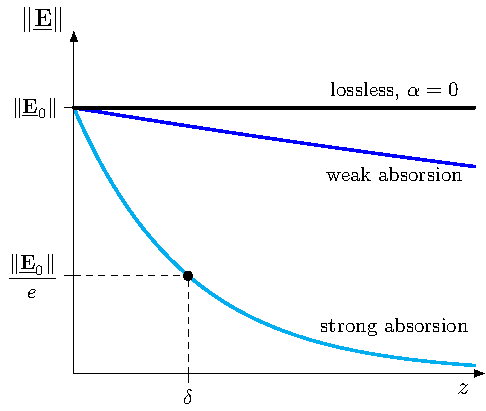
\includegraphics[width=\linewidth]{img/1/Skin-depth.pdf}
        \caption{Amplitude máxima de oscilação em função da distância de propagação~\protect\cite{silveirinha2023}. Escolheu-se $z$ para o exemplo.}
    \end{figure}
\end{minipage}\hfill
\begin{minipage}[b]{0.515\linewidth}
    O módulo da amplitude máxima de oscilação decai exponencialmente com a distância de propagação. Isto segue da definição em \eqref{eq:campos-onda-lossy-media}, onde $\mathbf{\underline{E}}_0$ é multiplicado pelos fatores
    \begin{equation*}
        e^{-\alpha \mathbf{\hat{d}} \cdot \mathbf{r}} \;\text{(regime exponencial)},
        \;\,
        e^{-j\beta \mathbf{\hat{d}} \cdot \mathbf{r}}
        \;\text{(regime sinusoidal)}.
    \end{equation*}
    O módulo $\norm{\mathbf{\underline{E}}}$ é obtido por:
    \begin{equation}
        \norm{\mathbf{\underline{E}}_0}\, e^{-\alpha \mathbf{\hat{d}} \cdot \mathbf{r}}
    \end{equation}
    Definimos a \emph{profundidade de penetração} (\emph{skin depth}) como:
    \begin{equation}
        \delta = \frac{1}{\alpha}
    \end{equation}
    A profundidade de penetração fornece uma estimativa aproximada da distância que uma onda pode penetrar dentro de um meio material antes de ser praticamente absorvida (i.e., decaia para ${\scriptsize \sim}37\%$ da amplitude original).
\end{minipage}


\begin{question}
    Para a frequência de oscilação de 1MHz, um material é caracterizado pela permitividade relativa $\epsilon_r = 2.5$ , pela permeabilidade relativa $\mu_r = 1$ , e pela condutividade $\sigma = 4 \times 10^{-5}$.\\[3pt]
    Determine: a) a tangente de perdas, b) a constante de atenuação, c) a constante de fase.
    
    \questionSep
    \textbf{Solução:} A tangente de perdas é definida em termos das partes real e imaginária da permitividade efetiva:
    $$
        \tan \theta = \frac{\epsilon''(\omega)}{\epsilon'(\omega)}\,\rightarrow\,
         \left\{
            \begin{aligned}
                &\epsilon'(\omega) =\epsilon_d'(\omega) = \epsilon_0\epsilon_r\\
                 &\epsilon''(\omega) =  \eqnmarkbox[violet]{pol-cunt}{\epsilon''_d(\omega)} + \frac{\sigma_c(\omega)}{\omega} = \frac{\sigma_c(\omega)}{\omega}
            \end{aligned}\right.
    $$
    \annotate[yshift=-0.1em]{below, label above}{pol-cunt}{Omitimos a componente da polarização}

    Assim,

    \vspace{-1.5em}
    $$
        \boxed{\tan \theta = \frac{\sigma}{\omega \epsilon_0 \epsilon_r} = 0.288}
    $$
    Ainda, $\gamma = jk = \alpha + j\beta$, logo:
    $$
        \begin{aligned}
            k = \omega\sqrt{\mu(\omega)\epsilon(\omega)} = \sqrt{\mu(\omega)\epsilon_d'(\omega)}\cdot\sqrt{1 - j\tan \theta} &= 0.0334 - j4.7\times 10^{-3} \; [\text{m}^{-1}]\\
            \gamma = jk &= \eqnmarkbox[violet]{fuck-waffle}{4.7\times 10^{-3} + j0.0334}
        \end{aligned}
    $$
    \annotate[yshift=-0.1em]{below, label above}{fuck-waffle}{$\alpha + j\beta$, respetivamente}
\end{question}
%//==============================--@--==============================//%
\clearpage
\subsubsection{Bons condutores e Bons Dielétricos}
Consideremos a dispersão de $\epsilon(\omega)$ e $\mu(\omega)$ negligenciável de forma a podermos escrever a constante de propagação e a impedância intrínseca da onda da seguinte forma:
\begin{align}
        \gamma &= j\omega\sqrt{\mu\left(\epsilon + \frac{\sigma}{j\omega}\right)} = j\omega\sqrt{\mu\epsilon}\eqnmarkbox[blue]{tan1}{\sqrt{1+\frac{\sigma}{j\omega\epsilon}}}\label{eq:gamma-nd}\\
        \eta &= \sqrt{\frac{\mu}{\epsilon + \frac{\sigma}{j\omega}}} = \sqrt{\frac{\mu}{\epsilon}}\frac{1}{\eqnmarkbox[blue]{tan2}{\sqrt{1+\frac{\sigma}{j\omega\epsilon}}}}\label{eq:eta}
\end{align}

\annotatetwo[yshift=-1cm,xshift=0cm]{below,right, label below}{tan1}{tan2}{Tanto a impedância quanto a constante de propagação\\ são governadas pelo parâmetro $\sqrt{1+\frac{\sigma}{j\omega\epsilon}}$}

\vspace{1.1em}
\begin{itemize}
    \item Caso $\sigma = 0$ o material torna-se não dispersivo e é dito \textit{dielétrico perfeito}.

    \item Caso $\sigma \neq 0$ mas $\sigma/\omega\epsilon \ll 1$ o material é dito \textit{bom dielétrico}. \eqref{eq:gamma-nd} e \eqref{eq:eta} podem ser escritas como
    \begin{equation}
        \gamma_{\text{good dielectric}} \approx \boxed{\dfrac{\sigma}{2}\sqrt{\frac{\mu}{\epsilon}} + j\frac{\omega}{c_0}\sqrt{\mu_r\epsilon_r}}\quad
        \eta_{\text{good dielectric}} \approx \boxed{\sqrt{\frac{\mu}{\epsilon}}\left(1+j\frac{\sigma}{2\omega\epsilon}\right)}
    \end{equation}

    \item Caso $\sigma/\omega\epsilon \gg 1$ o material é dito \textit{bom condutor} e: 
    \begin{equation}
        \gamma_{\text{good conductor}} \approx \boxed{\sqrt{\frac{\sigma\omega\mu}{2}}(1+j)}\qquad
        \eta_{\text{good conductor}} \approx \boxed{\sqrt{\frac{\omega\mu}{2\sigma}}(1+j)}
    \end{equation}
\end{itemize}

\vspace{-1em}
\begin{question}
    Um forno de micro-ondas trabalha à frequência de 2.5GHz. Nesta frequência um bife de lombo tem a permitividade complexa $30(1 - j0.3)\epsilon_0$.\\[3pt] 
    a) Qual o comprimento das micro-ondas no bife?\\[3pt] 
    b) Qual a profundidade de penetração (pelicular) das micro-ondas no bife?\\[3pt] 
    c) Se o bife é colocado num prato de plástico com $\epsilon=(1.1-j2\times10^{-4})\epsilon_0$ e espessura $3$mm, explique como este procedimento afeta o aquecimento do bife pelas micro-ondas.
    
    \questionSep
    \textbf{Solução}: Admitimos que:

    \vspace{-1.5em}
    $$
        \lambda = \frac{2\pi}{\beta}\qquad \beta = \Re\{k\}
    $$
    Por sua vez, recorrendo ao cálculo de $k$, para o qual $k = \beta - j\alpha$ (por definição)
    $$
        k = \omega\sqrt{\mu(\omega)\epsilon(\omega)}
        = \omega\sqrt{\mu_0\cdot 30(1 - j0.3)\epsilon_0} = 289.89 - j42.55
    $$
    Finalmente:

    \vspace{-1.5em}
    $$
        \lambda = \frac{2\pi}{\beta} = 21.67\,\text{mm}
    $$
    A profundida de penetração é dada por:

    \vspace{-1em}
    $$
        \delta = \frac{1}{\alpha} = 2.35\,\text{cm}
    $$
    Assumindo agora que $\epsilon=(1.1-j2\times10^{-4})\epsilon_0$ admitimos que
    $$
        \tan\theta = \frac{\sigma}{\omega\epsilon} = \frac{2\times 10^{-3}}{1.1} \ll 1\quad \text{(bom dielétrico)}\;\rightarrow\;
         \left\{
            \begin{aligned}
                 \gamma &\approx \eqnmarkbox[violet]{gamma}{\frac{\sigma}{2}\sqrt{\frac{\mu}{\epsilon}} + j\frac{\omega}{c_0}\sqrt{\mu_r\epsilon_r}}\\
                 \delta &= \frac{1}{\alpha} = 200\,\text{m}
            \end{aligned}\right.
    $$
    \annotate[yshift=2mm]{above, label above}{gamma}{$\alpha + j\beta,\;\alpha = 5\times10^{-3}$}

    Como o prato possui apenas 3 mm e $\delta = 200$m. A dissipação de energia é negligenciável, i.e, há baixa absorção/reflexão de energia pelo prato. O procedimento não afeta significativamente o aquecimento do bife.
\end{question}
%//==============================--@--==============================//%
\clearpage
\subsection{Polarização das Ondas}

Uma oscilação do campo eletromagnético não é totalmente determinada pela amplitude do campo. Devido à natureza vetorial do campo, existe um grau de liberdade adicional relacionado com a direção do espaço ao longo da qual o campo oscila. Este grau de liberdade é conhecido como a \emph{polarização do campo}.

A curva fechada determinada pela evolução temporal de $\mathbf{E}(t) = \Re\{ \mathbf{\underline{E}}e^{j\omega t} \}$. num ciclo completo de tempo (com período $T = 2\pi / \omega$) é a \emph{curva de polarização}. É simples demonstrar que a curva de polarização é sempre planar, uma vez que está no plano gerado pelos vetores ortogonais $\mathbf{E'} = \Re\{ \mathbf{\underline{E}} \}$ e $\mathbf{E''} = \Im\{ \mathbf{\underline{E}} \}$.

As propriedades de polarização da onda plana são determinadas pelas magnitudes relativas e fases das constantes complexas $\underline{A}$ e $\underline{B}$. Escrevendo-as nas suas formas polares $\underline{A} = A e^{j\phi_A}$ e $\underline{B} = B e^{j\phi_B}$, onde $A$ e $B$ são magnitudes positivas, obtemos:
\begin{equation}
    \begin{aligned}
        \mathbf{\underline{E}} &= \bigl(\underline{A} \mathbf{\hat{y}} + \underline{B} \mathbf{\hat{x}}\bigl)e^{-jkz}\\
        &= \left[A e^{j\phi_A}\mathbf{\hat{y}} + B e^{j\phi_B}\mathbf{\hat{x}}\right]e^{-jkz}
    \end{aligned}
\end{equation}

Extraindo a parte real e definindo $\mathbf{E}(z,t) = \Re\{\mathbf{\underline{E}}e^{j\omega t}\} = E_x(z,t) \mathbf{\hat{x}} + E_y(z,t) \mathbf{\hat{y}}$, encontramos as componentes reais em $x$ e $y$:
\begin{equation}
    \begin{aligned}
        E_y(z,t) &= A \cos(\omega t - kz + \phi_A)\\
        E_x(z,t) &= B \cos(\omega t - kz + \phi_B)
    \end{aligned}
\end{equation}
Para determinar a polarização da onda, consideramos a dependência temporal destes campos num ponto fixo ao longo do eixo $z$, digamos em $z = 0$:
\begin{equation}
    \begin{aligned}
        E_y(t) &= A \cos(\omega t + \phi_A)\\
        E_x(t) &= B \cos(\omega t + \phi_B)
    \end{aligned}
\end{equation}
Definimos a fase relativa $\phi = \phi_A - \phi_B$. Após alguma manipulação algébrica obtemos uma equação quadrática para as componentes $E_x$ e $E_y$, que descreve uma elipse no plano $E_x,\,E_y$:
\begin{equation}
    \left( \frac{E_y(t)}{B} \right)^2 \sin^2 \phi_A + \left( \frac{E_x(t)}{A} \right)^2 \sin^2 \phi_B - 2 \cos \phi \frac{E_x(t)E_y(t)}{AB} = \sin^2 \phi
\end{equation}

A trajetória do campo obtém-se através da omissão de $t$. A expressão  é simplificada para% fofinho, estou aqui
\begin{equation}\label{eq:polarization-eq} 
     \eqnmarkbox[blue]{pol}{\frac{E_x^2}{A^2} + \frac{E_y^2}{B^2} - 2 \cos \phi\, \frac{E_xE_y}{AB} = \sin^2 \phi}
\end{equation}
\annotate[yshift=-0.5em]{below, label above}{pol}{Elipse de polarização}

\begin{check}
    Dependendo dos valores das três quantidades ${A, B, \phi}$, esta elipse de polarização pode ser uma elipse, um círculo ou uma linha reta. 

    \begin{figure}[H]
        \centering
        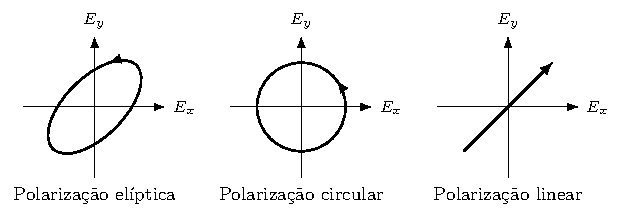
\includegraphics[width=0.75\linewidth]{img/1/Polarization.pdf}
        \caption{Tipos de polarização.}
    \end{figure}
\end{check}
%//==============================--@--==============================//%
\clearpage
Para obter a \textit{polarização linear}, definimos $\phi = 0$ ou $\phi = \pi$, o que corresponde a $\phi_A = \phi_B = 0$ ou $\phi_A = 0, \phi_B = -\pi$, de modo que as amplitudes dos fasores sejam $\mathbf{\underline{E}}_0 = \mathbf{\hat{y}}\underline{A} \pm \mathbf{\hat{x}}\underline{B}$. A Eq. \eqref{eq:polarization-eq} degenera em:
\begin{equation}
    \dfrac{E_{x}^2}{B^2} + \dfrac{E_{y}^2}{A^2} \pm \dfrac{2E_{x}E_{y}}{AB} = 0\,\rightarrow\, 
    \boxed{\left(\dfrac{E_{x}}{B} + \dfrac{E_{y}}{A}\right)^2 = 0}
\end{equation}
e consequentemente,
\begin{equation}
    \eqnmarkbox[blue]{lin}{E_{y} = \pm \dfrac{A}{B}E_{x}}
\end{equation}
\annotate[yshift=-0.1em]{below, label above}{lin}{reta de declive $\pm B/A$}

Para obter \textit{polarização circular}, definimos $A = B = R$ e $\phi = \pm \pi/2$. Neste caso, a elipse de polarização torna-se a equação de uma circunferência:
\begin{equation}
    \frac{E_{x}^2}{B^2} + \frac{E_{y}^2}{A^2} = 1
    \implies \eqnmarkbox[blue]{circ}{E_{x}^2 + E_{y}^2 = R^2}
\end{equation}
O sentido de rotação, em conjunto com a direção de propagação, define a polarização circular à esquerda/direita. Para o caso, $ \phi_a = -\pi/2 $ e $ \phi_b = 0 $, temos $\phi = \phi_a - \phi_b = -\pi/2$ e amplitude complexa $ \mathbf{\underline{E}}_0 = A(\mathbf{\hat{x}} - j\mathbf{\hat{y}}) $.

\vspace{-0.75em}
\begin{minipage}[c]{0.3\linewidth}
    \begin{figure}[H]
        \centering
        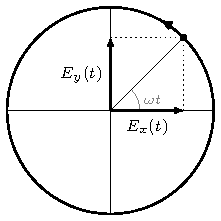
\includegraphics[width=0.915\linewidth]{img/1/Circular-polarization.pdf}
        \caption{Polarização circular.}
    \end{figure}
\end{minipage}\hfil
\begin{minipage}[c]{0.65\linewidth}
    Então,
     \begin{equation*}
        \begin{aligned}
            E_{x}(t) &= A \cos(\omega t)\\
            E_{y}(t) &= A \cos(\omega t - \pi/2) = A \sin(\omega t)
        \end{aligned}
    \end{equation*}
    Para determinar o sentido de rotação recorremos à evolução temporal do campo elétrico na curva de polarização. Calculando $\mathbf{E}(t=0)$ e $\mathbf{E}(t=0^+)$:
    \begin{equation*}
        t = 0: \, \left\{
        \begin{aligned}
            E_{x}(0) &= A\\
            E_{y}(0) &= 0
        \end{aligned}\right.
        \qquad
        t = 0^+: \, \left\{
        \begin{aligned}
            E_{x}(0^+) &\approx A\\
            E_{y}(0^+) &\approx 0^+
        \end{aligned}\right.
    \end{equation*}
    O campo gira no sentido anti-horário no plano $xy$.
\end{minipage}

\begin{warning}
    Para decidir se a polarização circular é à direita ou à esquerda, usamos a convenção da IEEE~\cite{ieee1983terms}: 
    \begin{itemize}
        \item Enrolar os dedos da mão esquerda e direita em punho e apontar ambos os polegares na direção de propagação. 
        \item Se os dedos da mão direita (esquerda) enrolam na direção de rotação do campo elétrico, então a polarização é à direita (esquerda).
    \end{itemize}
    Portanto, neste exemplo, como o campo se move na direção de $z$ e gira no sentido anti-horário, a polarização será à direita.
\end{warning}

Caso $A \neq B$ e $\phi = \pm \pi/2$, obtemos uma \textit{polarização elíptica}\footnote{A análise da orientação da polarização é análoga à da polarização circular.}. A Eq. \eqref{eq:polarization-eq} será agora:
\begin{equation}
    \eqnmarkbox[blue]{eli}{\frac{E_{x}^2}{B^2} + \frac{E_{y}^2}{A^2} = 1}
\end{equation}

\subsubsection{Rácio de Polarização}

Em resumo, definindo a amplitude complexa $\mathbf{\underline{E}} = \underline{E}_1 \mathbf{\hat{u}}_1 + \underline{E}_2 \mathbf{\hat{u}}_2$, tal que o par de versores ($\mathbf{\hat{u}}_1$, $\mathbf{\hat{u}}_2$) forme uma base ortogonal do plano perpendicular à direção de propagação $\mathbf{\hat{d}} = \mathbf{\hat{u}}_1 \times \mathbf{\hat{u}}_2$, podemos estabelecer o \textit{rácio de polarização}:
\begin{equation}
    p = \frac{\underline{E}_2}{\underline{E}_1} \equiv \abs{p} e^{j\phi}
\end{equation}

\begin{check}
    A amplitude $\abs{p}$ e a fase $\phi$ da razão de polarização determinam completamente a polarização da onda de acordo com as seguintes regras:
    \begin{itemize}
        \item Se $\phi = \pm \pi/2$ e $\abs{p} = 1$, a onda tem polarização circular.
        \item Se $\phi = 0$ ou $\phi = \pi$ ou $\abs{p} = 0$ ou $\abs{p} = \infty$, a onda tem polarização linear.
        \item Se nenhuma das condições acima se verifica, então o estado de polarização é elíptico.
    \end{itemize}
    Além disto, o ângulo $\phi$ controla o sentido de rotação, de modo que para $0 < \phi < \pi$ a onda está polarizada para a esquerda, enquanto para $-\pi < \phi < 0$ a onda está polarizada para a direita. É de sublinhar que este resultado só é válido quando a direção de propagação é $\mathbf{\hat{d}} = \mathbf{\hat{u}}_1 \times \mathbf{\hat{u}}_2$.
\end{check}

A mesma análise poderá ser feita com o campo $\mathbf{H}$, naturalmente.

%//==============================--@--==============================//%
\vfill
\begin{question}
    O fasor do campo magnético associado a uma onda plana e uniforme é dado por:
    $$
        \mathbf{\underline{H}} = \frac{10^{-3}}{120\pi}\left(\mathbf{\hat{x} - j\mathbf{\hat{y}}}\right)e^{jky}
    $$
    a) Determine o estado de polarização da onda.\\[3pt]
    b) Diga qual o sentido de rotação.\\[3pt]
    c) Esboce a curva de polarização.

    \questionSep
    \textbf{Solução}: Extraindo a parte real e definindo $\mathbf{H}(y,t) = \Re\{\mathbf{\underline{H}} e^{j\omega t}\} = H_x(y,t) \mathbf{\hat{x}} + H_z(y,t) \mathbf{\hat{z}}$, encontramos as componentes reais em $x$ e $y$:
    \begin{equation}
        \begin{aligned}
            H_z(y,t) &= \frac{10^{-3}}{120\pi} \cos\left(\omega t + ky -\pi/2\right)\\[1pt]
            H_x(y,t) &= \frac{10^{-3}}{120\pi} \cos(\omega t + ky)
        \end{aligned}
    \end{equation}
    Para determinar a polarização da onda, consideramos a dependência temporal do campo num ponto fixo ao longo do eixo $y$, digamos em $y = 0$:
    \begin{equation}
        \begin{aligned}
            H_z(t) &= \frac{10^{-3}}{120\pi} \cos\left(\omega t -\pi/2\right) = \frac{10^{-3}}{120\pi}\sin(\omega t)\\[1pt]
            H_x(t) &= \frac{10^{-3}}{120\pi} \cos(\omega t)
        \end{aligned}
    \end{equation}
    Como $\phi = 0 - (-\pi/2) = \pi/2$ a equação de polarização é dada por:
    $$
       H_{x}^2 + H_{z}^2 = 10^{-6}/(120\pi)^2\quad \text{(Polarização circular)}
    $$
    Para determinar o sentido de rotação recorremos à evolução temporal do campo elétrico na curva de polarização. Calculando $\mathbf{H}(t=0)$ e $\mathbf{H}(t=0^+)$:
    \begin{equation*}
        t = 0: \, \left\{
        \begin{aligned}
            H_{x}(0) &= \frac{10^{-3}}{120\pi}\\[1pt]
            H_{z}(0) &= 0
        \end{aligned}\right.
        \qquad
        t = 0^+: \, \left\{
        \begin{aligned}
            H_{x}(0^+) &\approx \frac{10^{-3}}{120\pi}\\[1pt]
            H_{z}(0^+) &\approx 0^+
        \end{aligned}\right.
    \end{equation*}
    O campo gira no sentido anti-horário no plano $xz$. A polarização é à direita por congruência com a regra da mão direita (nomeadamente, os dedos da mão direita enrolam na direção de rotação do campo magnética, com o polegar a apontar na direção de propagação).
    
    \qed
\end{question}
%//==============================--@--==============================//%